\documentclass[14pt,xcolor=pdftex,dvipsnames,table]{beamer}\usepackage[]{graphicx}\usepackage[]{color}
%% maxwidth is the original width if it is less than linewidth
%% otherwise use linewidth (to make sure the graphics do not exceed the margin)
\makeatletter
\def\maxwidth{ %
  \ifdim\Gin@nat@width>\linewidth
    \linewidth
  \else
    \Gin@nat@width
  \fi
}
\makeatother

\definecolor{fgcolor}{rgb}{0.345, 0.345, 0.345}
\newcommand{\hlnum}[1]{\textcolor[rgb]{0.686,0.059,0.569}{#1}}%
\newcommand{\hlstr}[1]{\textcolor[rgb]{0.192,0.494,0.8}{#1}}%
\newcommand{\hlcom}[1]{\textcolor[rgb]{0.678,0.584,0.686}{\textit{#1}}}%
\newcommand{\hlopt}[1]{\textcolor[rgb]{0,0,0}{#1}}%
\newcommand{\hlstd}[1]{\textcolor[rgb]{0.345,0.345,0.345}{#1}}%
\newcommand{\hlkwa}[1]{\textcolor[rgb]{0.161,0.373,0.58}{\textbf{#1}}}%
\newcommand{\hlkwb}[1]{\textcolor[rgb]{0.69,0.353,0.396}{#1}}%
\newcommand{\hlkwc}[1]{\textcolor[rgb]{0.333,0.667,0.333}{#1}}%
\newcommand{\hlkwd}[1]{\textcolor[rgb]{0.737,0.353,0.396}{\textbf{#1}}}%

\usepackage{framed}
\makeatletter
\newenvironment{kframe}{%
 \def\at@end@of@kframe{}%
 \ifinner\ifhmode%
  \def\at@end@of@kframe{\end{minipage}}%
  \begin{minipage}{\columnwidth}%
 \fi\fi%
 \def\FrameCommand##1{\hskip\@totalleftmargin \hskip-\fboxsep
 \colorbox{shadecolor}{##1}\hskip-\fboxsep
     % There is no \\@totalrightmargin, so:
     \hskip-\linewidth \hskip-\@totalleftmargin \hskip\columnwidth}%
 \MakeFramed {\advance\hsize-\width
   \@totalleftmargin\z@ \linewidth\hsize
   \@setminipage}}%
 {\par\unskip\endMakeFramed%
 \at@end@of@kframe}
\makeatother

\definecolor{shadecolor}{rgb}{.97, .97, .97}
\definecolor{messagecolor}{rgb}{0, 0, 0}
\definecolor{warningcolor}{rgb}{1, 0, 1}
\definecolor{errorcolor}{rgb}{1, 0, 0}
\newenvironment{knitrout}{}{} % an empty environment to be redefined in TeX

\usepackage{alltt}

% Specify theme
\usetheme{Madrid}
% See deic.uab.es/~iblanes/beamer_gallery/index_by_theme.html for other themes
\usepackage{caption}
\usepackage{tikz}
\usepackage{multirow}
% Specify base color
\usecolortheme[named=OliveGreen]{structure}
% See http://goo.gl/p0Phn for other colors

% Specify other colors and options as required
\setbeamercolor{alerted text}{fg=Maroon}
\setbeamertemplate{items}[square]

% Title and author information
\title{Monopoly-competition}
\author{Rob Hayward}
\IfFileExists{upquote.sty}{\usepackage{upquote}}{}
\begin{document}

\begin{frame}
\titlepage
\end{frame}


\section{Refresh output and costs}
\section{Monopoly vs competition}



%[<+-| alert@+>]


\begin{frame}{Average Costs}
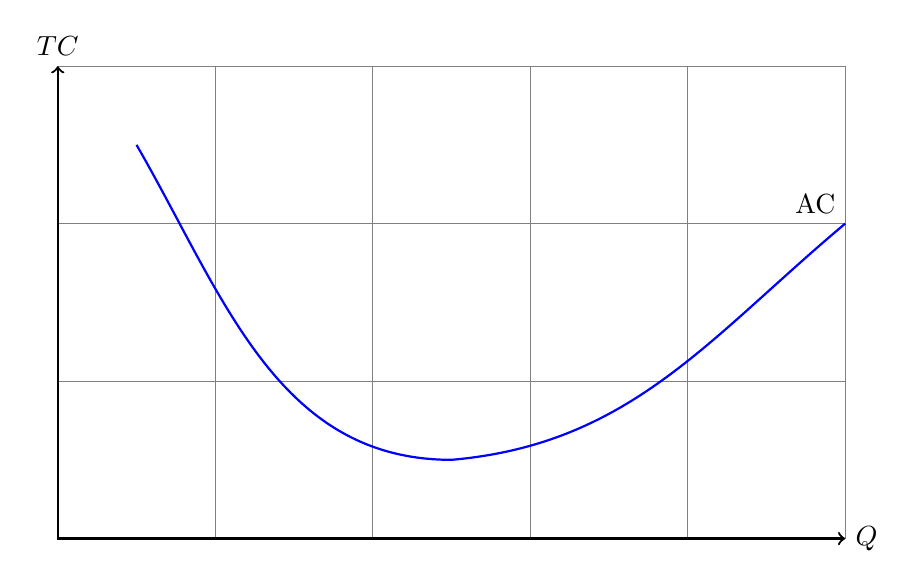
\begin{tikzpicture}[scale = 2]
\draw[very thin, color = gray](0, 0) grid (5, 3);
\draw [<->, thick] (0, 3) node (yaxis) [above] {$TC$} 
  |- (5, 0) node (xaxis) [right] {$Q$};
\node at (5, 2) [above left] {AC};
\draw[thick, color = blue] (0.5, 2.5) to [out = -60, in = 180] (2.5, 0.5) to [out = 5, in = 220] (5, 2);
%\draw[domain = 0.1:3.9, color = blue] plot(\x, {2 - 0.5*\x});
\end{tikzpicture}
\end{frame}

\begin{frame}{Shape of average cost}
The average cost curve is U shaped because
\begin{itemize}[<+-| alert@+>]
\item Average costs initially fall with specialisation
\item Average costs initially fall because fixed costs are spread
\item Average costs eventually rise because of \emph{diminishing returns} in the short-run
\item Average costs eventaully rise because of \emph{diseconimies of scale} in the long-run
\end{itemize}
\end{frame}

\begin{frame}{Marginal costs}
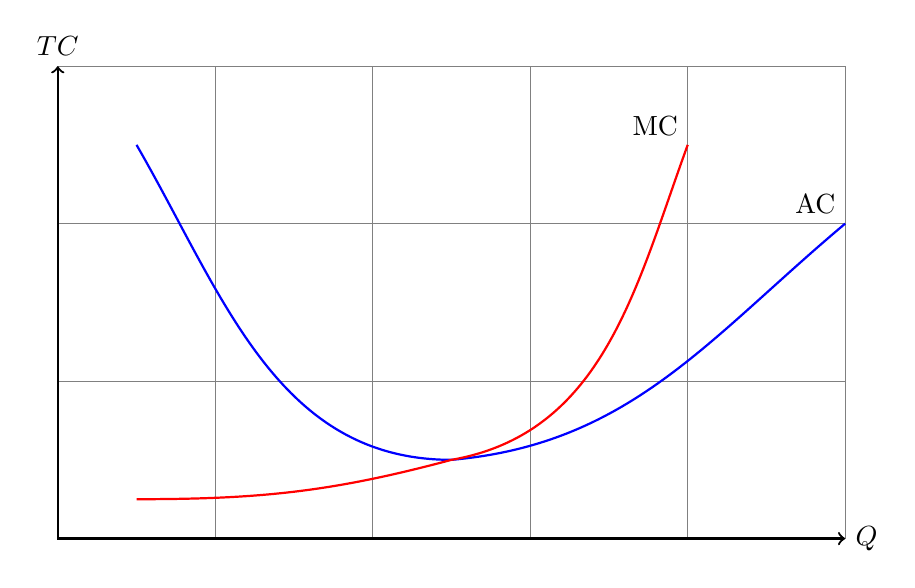
\begin{tikzpicture}[scale = 2]
\draw[very thin, color = gray](0, 0) grid (5, 3);
\draw [<->, thick] (0, 3) node (yaxis) [above] {$TC$} 
  |- (5, 0) node (xaxis) [right] {$Q$};
\node at (5, 2) [above left] {AC};
\node at (4, 2.5) [above left] {MC};
\draw[thick, color = blue] (0.5, 2.5) to [out = -60, in = 180] (2.5, 0.5) to [out = 5, in = 220] (5, 2);
\draw[thick, color = red] (0.5, 0.25) to [out = 0, in = 195] (2.5, 0.5) to [out = 10, in = 250] (4, 2.5);
%\draw[domain = 0.1:3.9, color = blue] plot(\x, {2 - 0.5*\x});
\end{tikzpicture}
\end{frame}

\begin{frame}{Shape and position of the marginal cost}
The average cost curve is U shaped because
\begin{itemize}[<+-| alert@+>]
\item The marginal cost is the cost of one more unit of output
\item The marginal cost is below the average cost while average cost is falling
\item The marginal cost is above the average  cost while the average cost is rising
\item The marginal cost cuts the average cost at the lowest point on the average cost
\end{itemize}
\end{frame}

\begin{frame}{Perfect Competition}
In a perflectly competitive market, the marginal cost curve is the firm supply curve
\begin{columns}[T]
\begin{column}{.48\textwidth}
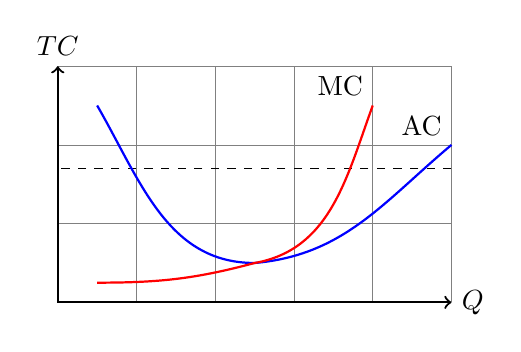
\begin{tikzpicture}
\draw[very thin, color = gray](0, 0) grid (5, 3);
\draw [<->, thick] (0, 3) node (yaxis) [above] {$TC$} 
  |- (5, 0) node (xaxis) [right] {$Q$};
\node at (5, 2) [above left] {AC};
\node at (4, 2.5) [above left] {MC};
\draw [dashed] (5, 1.70) to (0, 1.70);
\draw[thick, color = blue] (0.5, 2.5) to [out = -60, in = 180] (2.5, 0.5) to [out = 5, in = 220] (5, 2);
\draw[thick, color = red] (0.5, 0.25) to [out = 0, in = 195] (2.5, 0.5) to [out = 10, in = 250] (4, 2.5);
%\draw[domain = 0.1:3.9, color = blue] plot(\x, {2 - 0.5*\x});
\end{tikzpicture}
\end{column}
\begin{column}{.48\textwidth}
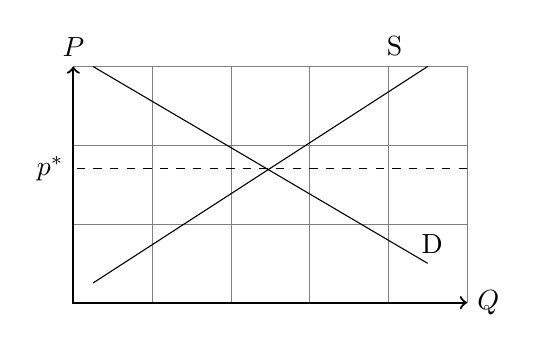
\begin{tikzpicture}
\draw[very thin, color = gray](0, 0) grid (5, 3);
\draw [<->, thick] (0, 3) node (yaxis) [above] {$P$} 
  |- (5, 0) node (xaxis) [right] {$Q$};
\node at (4.3, 0.5) [above right] {D};
\node at (4.3, 3.5) [below left] {S};
\node at (0, 1.70) [left] {$p^*$};
\draw (0.25, 3) to (4.5, 0.5);
\draw (0.25, 0.25) to (4.5, 3);
\draw [dashed] (5, 1.70) to (0, 1.70);
%\draw[domain = 0.1:3.9, color = blue] plot(\x, {2 - 0.5*\x});
\end{tikzpicture}
\end{column}
\end{columns}
Equilibrium price = $P^* = AR = MR$
\end{frame}

\begin{frame}{Profit maximisation}
Prfit maximised at MR = MC
\begin{columns}[T]
\begin{column}{.48\textwidth}
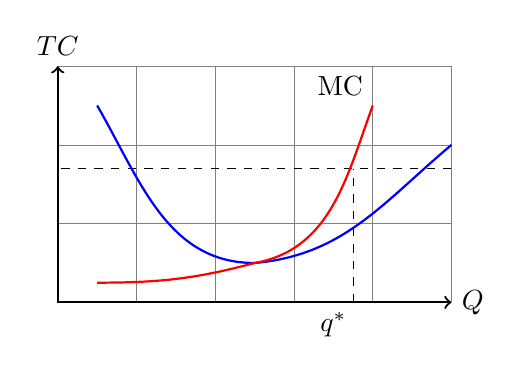
\begin{tikzpicture}
\draw[very thin, color = gray](0, 0) grid (5, 3);
\draw [<->, thick] (0, 3) node (yaxis) [above] {$TC$} 
  |- (5, 0) node (xaxis) [right] {$Q$};
%\node at (5, 2) [above left] {AC};
\node at (4, 2.5) [above left] {MC};
\draw [dashed] (5, 1.70) to (0, 1.70);
\draw [dashed] (3.75, 0) to (3.75, 1.70);
\node at (3.5, 0) [below] {$q^*$};
\draw[thick, color = blue] (0.5, 2.5) to [out = -60, in = 180] (2.5, 0.5) to [out = 5, in = 220] (5, 2);
\draw[thick, color = red] (0.5, 0.25) to [out = 0, in = 195] (2.5, 0.5) to [out = 10, in = 250] (4, 2.5);
%\draw[domain = 0.1:3.9, color = blue] plot(\x, {2 - 0.5*\x});
\end{tikzpicture}
\end{column}
\begin{column}{.48\textwidth}
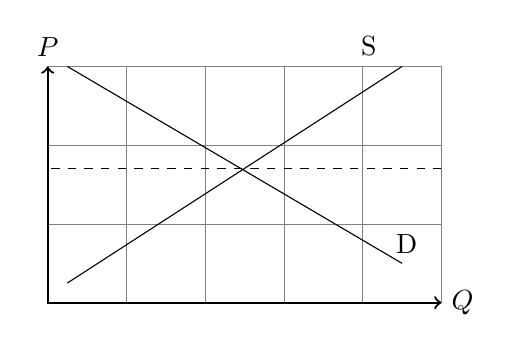
\begin{tikzpicture}
\draw[very thin, color = gray](0, 0) grid (5, 3);
\draw [<->, thick] (0, 3) node (yaxis) [above] {$P$} 
  |- (5, 0) node (xaxis) [right] {$Q$};
\node at (4.3, 0.5) [above right] {D};
\node at (4.3, 3.5) [below left] {S};
\draw (0.25, 3) to (4.5, 0.5);
\draw (0.25, 0.25) to (4.5, 3);
\draw [dashed] (5, 1.70) to (0, 1.70);
%\draw[domain = 0.1:3.9, color = blue] plot(\x, {2 - 0.5*\x});
\end{tikzpicture}
\end{column}
\end{columns}
Profit-maximising output moves along the MC curve
\end{frame}

\begin{frame}{Supply increase}
Prfit maximised at MR = MC
\begin{columns}[T]
\begin{column}{.48\textwidth}
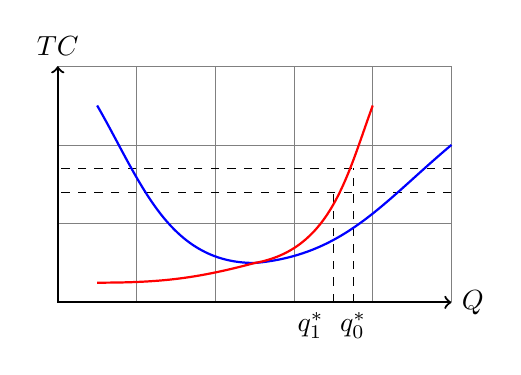
\begin{tikzpicture}
\draw[very thin, color = gray](0, 0) grid (5, 3);
\draw [<->, thick] (0, 3) node (yaxis) [above] {$TC$} 
  |- (5, 0) node (xaxis) [right] {$Q$};
%\node at (5, 2) [above left] {AC};
%\node at (4, 2.5) [above left] {MC};
\draw [dashed] (5, 1.70) to (0, 1.70);
\draw [dashed] (5, 1.40) to (0, 1.40);
\draw [dashed] (3.75, 0) to (3.75, 1.70);
\draw [dashed] (3.50, 0) to (3.50, 1.40);
\node at (3.75, 0) [below] {$q_0^*$};
\node at (3.50, 0) [below left] {$q_1^*$};
\draw[thick, color = blue] (0.5, 2.5) to [out = -60, in = 180] (2.5, 0.5) to [out = 5, in = 220] (5, 2);
\draw[thick, color = red] (0.5, 0.25) to [out = 0, in = 195] (2.5, 0.5) to [out = 10, in = 250] (4, 2.5);
%\draw[domain = 0.1:3.9, color = blue] plot(\x, {2 - 0.5*\x});
\end{tikzpicture}
\end{column}
\begin{column}{.48\textwidth}
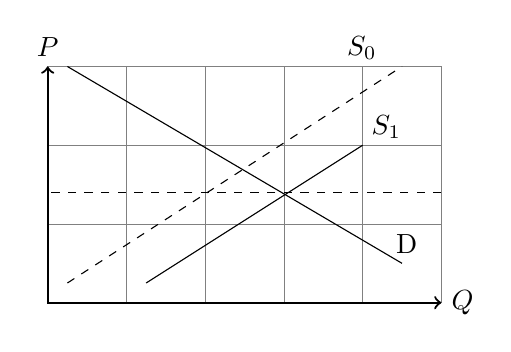
\begin{tikzpicture}
\draw[very thin, color = gray](0, 0) grid (5, 3);
\draw [<->, thick] (0, 3) node (yaxis) [above] {$P$} 
  |- (5, 0) node (xaxis) [right] {$Q$};
\node at (4.3, 0.5) [above right] {D};
\node at (4.3, 3.5) [below left] {$S_0$};
\node at (4.3, 2.5) [below] {$S_1$};
\draw (0.25, 3) to (4.5, 0.5);
\draw [dashed] (0.25, 0.25) to (4.5, 3);
\draw (1.25, 0.25) to (4.0, 2.0);
\draw [dashed] (5, 1.40) to (0, 1.40);
%\draw[domain = 0.1:3.9, color = blue] plot(\x, {2 - 0.5*\x});
\end{tikzpicture}
\end{column}
\end{columns}
Profit-maximising output moves along the MC curve
\end{frame}

\begin{frame}{Long-run Equilibrium}
\begin{columns}[T]
\begin{column}{.48\textwidth}
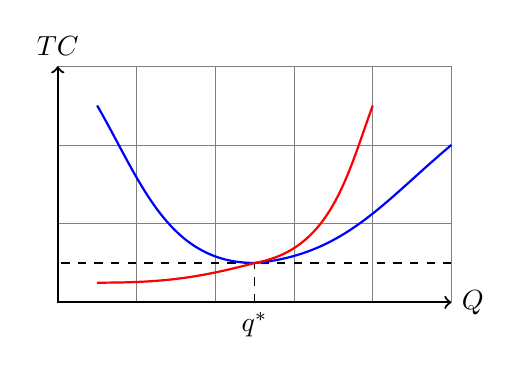
\begin{tikzpicture}
\draw[very thin, color = gray](0, 0) grid (5, 3);
\draw [<->, thick] (0, 3) node (yaxis) [above] {$TC$} 
  |- (5, 0) node (xaxis) [right] {$Q$};
%\node at (5, 2) [above left] {AC};
%\node at (4, 2.5) [above left] {MC};
\draw [dashed] (5, 0.5) to (0, 0.5);
%\draw [dashed] (5, 1.40) to (0, 1.40);
%\draw [dashed] (3.75, 0) to (3.75, 1.70);
\draw [dashed] (2.50, 0) to (2.50, 0.5);
\node at (2.5, 0) [below] {$q^*$};
\draw[thick, color = blue] (0.5, 2.5) to [out = -60, in = 180] (2.5, 0.5) to [out = 5, in = 220] (5, 2);
\draw[thick, color = red] (0.5, 0.25) to [out = 0, in = 195] (2.5, 0.5) to [out = 10, in = 250] (4, 2.5);
%\draw[domain = 0.1:3.9, color = blue] plot(\x, {2 - 0.5*\x});
\end{tikzpicture}
\end{column}
\begin{column}{.48\textwidth}
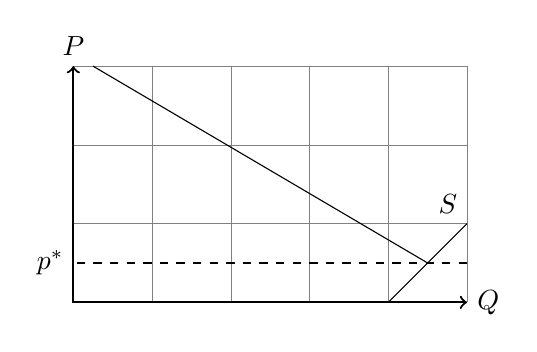
\begin{tikzpicture}
\draw[very thin, color = gray](0, 0) grid (5, 3);
\draw [<->, thick] (0, 3) node (yaxis) [above] {$P$} 
  |- (5, 0) node (xaxis) [right] {$Q$};
%\node at (4.3, 0.5) [above right] {D};
\node at (5, 1) [above left] {$S$};
\node at (0, 0.5) [left] {$p^*$};
%\node at (4.3, 2.5) [below] {$S_1$};
\draw (0.25, 3) to (4.5, 0.5);
%\draw [dashed] (0.25, 0.25) to (4.9, 2.8);
\draw (4, 0) to (5, 1);
\draw [dashed] (5, 0.5) to (0, 0.5);
%\draw[domain = 0.1:3.9, color = blue] plot(\x, {2 - 0.5*\x});
\end{tikzpicture}
\end{column}
\end{columns}
Long-run equilibrium when price is equal to the minimum on the average cost curve. 
\end{frame}

\begin{frame}{Monopoly}
For monopoly, the firm and the market are the same
There are barriers to entry
\begin{itemize}[<+-| alert@+>]
\item Government or regulatory
\item Patents or unique product 
\item Access to customers or materials
\item First-mover advantage
\item Threats
\item Agreements
\end{itemize}
\end{frame}

\begin{frame}{Price Discrimination}
%\includegraphics<1>[width=12cm, height=9cm]{"../Figures/train"}
\end{frame}



\end{document}
